\section{Discusión}

\subsection{Anomalías detectadas}

En primer lugar, cabe notar que en casi todos los casos la medición por RTT tiene una forma parecida: hay una cierta cantidad de hops que tienen RTTs muy similares y luego se da un salto significativo (donde el RTT aumenta al menos en un 30\%) hacia otro grupo de hops cercanos entre sí \textit{(en términos de RTT)}. Esto sucede dos o tres veces según la universidad elegida, y da la idea de que los RTTs de lugares cercanos son similares y cuánto más lejos se halle el destino mayor es el RTT, lo que coincide con la teoría y la intuición.


Dentro de estos grupos se ve que hay envíos de TTL superior con menor RTT \textit{(por ejemplo, para el TTL 6 se obtiene un RTT menor que el obtenido para el TTL 5)}, lo que no tiene sentido dado que recorren una mayor cantidad de hops. Esto es posiblemente consecuencia de promediar mediciones de rutas distintas y de diferente niveles de congestión de la red. En cada envío de paquetes no podemos asegurar que el estado de la red fuese el mismo, y por lo tanto, se están promediando rutas que pueden no tener las mismas características.


Otra anomalía con la que nos encontramos fue que si bien se nota que hay grupos 
cercanos por RTTs y ZRTTs muy parecidos, esto no parece coincidir con la información 
de geolocalización obtenida a partir de la IP. Esto probablemente provenga de un error 
de geolocalización que mencionamos en la sección del \textit{traceroute}. El servicio 
que provee las coordenadas a partir de una IP puede ocasionalmente devolver 
una localización que está asociada con un servicio proveedor que no está por donde 
realmente pasó el paquete. Esto se ve muy claro en el caso de Rusia y Australia 
(figuras \ref{rtt-aus}, \ref{zrtt-aus}, \ref{rtt-rus}, \ref{zrtt-rus}) donde el 
primer o segundo hop marcado como dentro de Estados Unidos tiene RTT y ZRTT muy 
similar a los obtenidos para los hops de Argentina, mientras que el siguiente denota 
un cambio importante y sería ahí donde se imaginaría que ocurrió el salto de más distancia. 
Creemos que esto es un error de localización y no que el salto ocurre allí donde 
los valores son tan parecidos a los argentinos.

\subsection{Identificación de enlaces submarinos}

En teoría, el RTT de aquellos enlaces que cubren muchos kilómetros debería ser evidentemente mayor que el de los enlaces más cercanos. En la práctica realizada, exceptuando los errores de localización o de experimentación mencionados, se pudo visualizar esta diferencia. El caso de Noruega es claro e interesante (figuras \ref{zrtt-nor} y \ref{rtt-nor}): En el gráfico de ZRTT se ve claramente el salto entre Uruguay y el Reino Unido, con una diferencia enorme en el valor standard del RTT. Observando el RTT, se puede ver que el tiempo se duplica entre uno y el otro. Y luego, si bien hay saltos dentro de Europa los RTTs se mantienen relativamente parecidos.

En el resto de los casos se pueden ver el mismo tipo de saltos numéricos significativos: todos los ejemplos muestran uno o dos puntos donde el RTT aumenta significativamente a partir de un hop y para todos los siguientes. En los gráficos de ZRTT se ve un cambio importante en uno o dos lugares, pero como decíamos antes, no siempre coincide con el cambio de país según la geolocalización. En los casos de Noruega (fig \ref{zrtt-nor}) y Australia (fig \ref{zrtt-aus}) esto se ve claro y coincide con la localización hallada. Creemos que en los otros dos también se observa, aún si la localización no está mostrando el momento correcto.

Sería posible armar una heurística para detectar estos saltos en los cambios más elevados del ZRTT. Pero hay que notar que las pruebas son muy sensibles al estado de la red, y hay cantidades de variables difíciles de predecir, como la congestión de la red y la variabilidad de las rutas posibles. %Creemos que en aquellos casos en que el ZRRT de un hop crezca con respecto al ZRTT del hop anterior en mas de $0.5$ podemos decir que dicho par de hops se corresponde con los dos extremos de un enlace submarino.

\textbf{Heurística propuesta}: Sea $rZRRT_i = ZRRT_i - ZRRT_{i+1}$. Entonces decimos que los hops $i$ e $i-1$ son los extremos de un enlace submarino sii $rZRRT \geq 0.5$.\\

Se puede ver que la heurística propuesta identifica correctamente los enlaces submarinos en los cuatro experimentos realizados (figuras \ref{zrtt-aus}, \ref{zrtt-nor}, \ref{zrtt-tok} y \ref{zrtt-rus}) mediante los siguiente gráficos del ZRTT relativo de cada hop con respecto al hop anterior:

\begin{figure}[H]
  \centering
    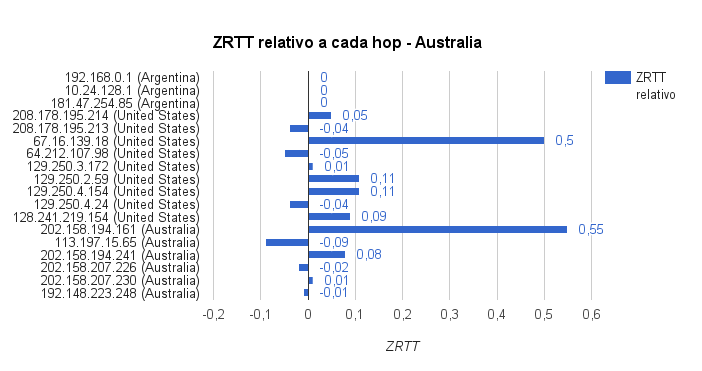
\includegraphics[width=1\textwidth]{../Experimentacion/rel-australia.png}
\end{figure}

Para llegar a Australia se utilizan dos enlaces submarinos: Argentina-EEUU y EEUU-Australia. Aplicando nuestra heuristica vemos que los pares de IP (208.178.195.213, 67.16.139.18) y (128.241.219.154, 202.158.194.161) son los extremos de los dos enlaces mencionadas, cada IP perteneciendo a uno de los piases del enlace \textit{(fácilmente deducible en función de la ruta)}

\begin{figure}[H]
  \centering
    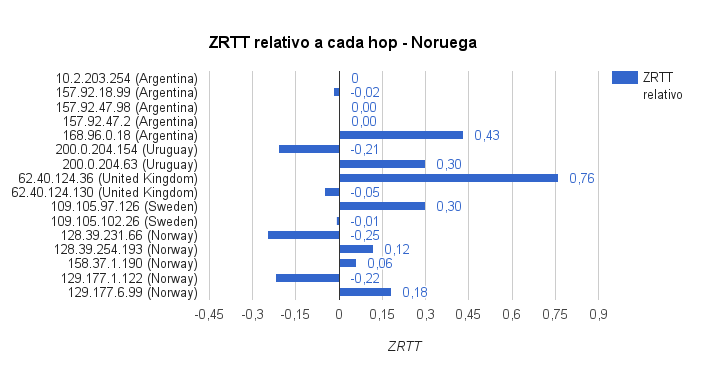
\includegraphics[width=1\textwidth]{../Experimentacion/rel-noruega.png}
\end{figure}

Aquí podemos ver que el único enlace utilizado: Uruguay-Reino Unido es claramente identificable por nuestra heurística dando como resultado el par (200.0.204.63, 62.40.124.130).

\begin{figure}[H]
  \centering
    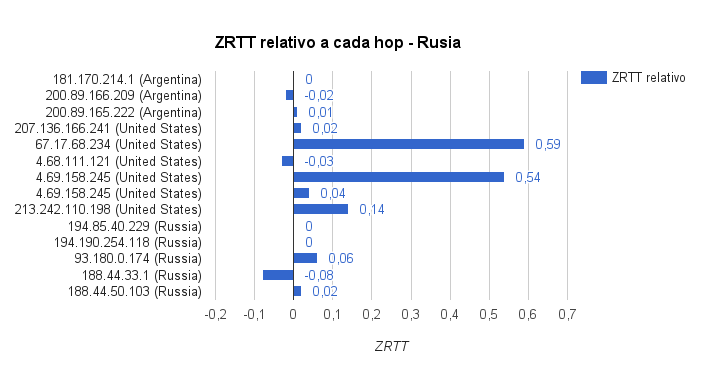
\includegraphics[width=1\textwidth]{../Experimentacion/rel-rusia.png}
\end{figure}

Aquí, al igual que sucedió en el caso de Australia se utilizan dos enlaces: Argentina-EEUU y EEUU-Rusia. Ambos son detectados por nuestra heurística.

\begin{figure}[H]
  \centering
    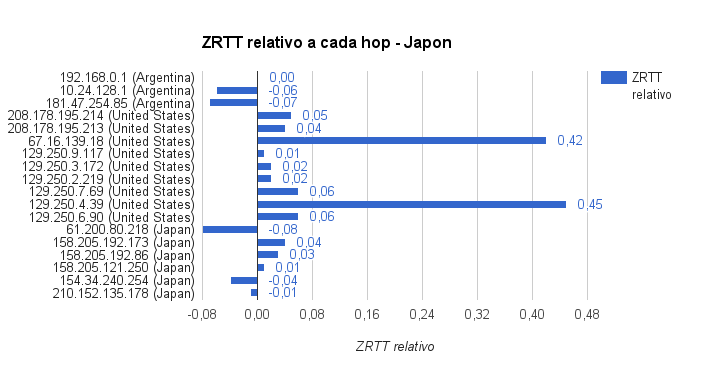
\includegraphics[width=1\textwidth]{../Experimentacion/rel-tokyo.png}
\end{figure}

Aquí también se utilizan dos enlaces: Argentina-EEUU y EEUU-Japón. A pesar de que ambos pares de hops son identificables a simple vista, nuestra heurística falla al detectarlos. Al ser una heurística es normal que existan casos en los que falle. En este caso en particular bastaría con mover el umbral a $0.4$ para detectar los enlaces, pero teniendo en cuenta que el resultado analizado es obtenido de una única ejecución del algoritmo de \textit{traceroute}, no lo creemos necesario. Muy probablemente si se realizara otra ejecución del traceroute, la heurística seria capaz de detectar ambos enlaces.

\subsection{Análisis del contraste con la realidad}

Es importante tener en cuenta al comparar los RTT calculados por \textit{ping} y los calculados por \textit{traceroute}, que este último sólo realiza un promedio entre tres muestras de RTT \textit{(las cuales pueden haber sido afectados por muchos factores de la red, o que el host destino haya retrasado intencionalmente el envío de la respuesta, aumentando el RTT en forma directa)}.

\begin{table}[H]
  \centering
    \begin{tabular}{lllll}
    \hline
    Universidad & RTT traceroute & RTT ping minimo & RTT ping maximo \\ \hline
    Australia - ACU &  418.61 ms  &  350.73 ms  &  356.06 ms \\
    Noruega - UIB   &  313.06 ms  &  270.23 ms  &  335.69 ms \\
  Japón - U-Tokyo &  381.23 ms  &  295.47 ms  &  315.45 ms \\
  Rusia - MSU     &  327.28 ms  &  347.15 ms  &  355.24 ms \\ \hline
    \end{tabular}
    \caption{Resultado del análisis de las muestras de RTTs}
  \label{fig:tabla-comp-rtt}
\end{table}


En el caso de Australia y Japón, los RTT obtenidos por \textit{traceroute} son, aproximadamente, un 20\% superiores al máximo valor obtenido por \textit{ping}.
En el caso de Noruega, el valor del RTT se encuentra en el intervalo definido por \textit{ping} y en el caso de Rusia el valor es cercano al mínino obtenido por \textit{ping}.


Puede observarse que en los experimentos, muchas veces, no sufrimos de pérdida de paquetes. Esto hace que el cálculo del throughput nos de el valor máximo teórico para el enlace. Este valor es significativamente superior que el obtenido en todos los casos en donde hubo pérdida de paquetes. En los casos donde hubo pérdida de paquetes, obtuvimos un throughput muy inferior al máximo valor teórico. Por ejemplo, en el experimento realizado contra la universidad de Noruega obtuvimos un throughput teórico de, aproximadamente 230 Kbytes por segundo. Pero, al tener una pérdida de paquetes de tan solo 0.67\% \textit{(aproximadamente, 7 paquetes perdidos de cada 1000 enviados)} el throughput disminuyo a 65 Kbytes por segundo, lo cual equivale a una perdida de, aproximadamente, el 70\% del throughput teórico.

Algo similar ocurre en el experimento realizado contra la universidad de Rusia, donde tenemos un throughput máximo teórico de, aproximadamente, 206 Kbytes por segundo y con una probabilidad de pérdida de paquetes del 4.67\% el throughput cae a 22 Kbytes por segundo, es decir, tenemos una pérdida del 90\% del throughput. Luego vemos que, aunque la probabilidad de pérdida de paquetes aumente al 5.7\%, el throughput solo disminuye en 2 Kbytes por segundo.

Esta fuerte disminución en el throughput cuando la probabilidad de pérdida de paquetes ni siquiera a alcanzado el 1\% se debe a la relación presente entre ambos en la fórmula de Mathis, de la forma: throughput $=$ $\frac{1}{\sqrt{PktLoss}}$. Entonces, la disminución del throughput con respecto al aumento de la probabilidad de pérdida de paquetes tendrá la siguiente forma:


\begin{figure}[H]
  \centering
    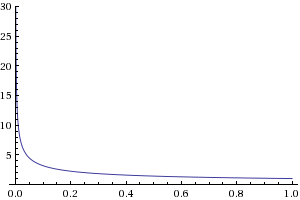
\includegraphics[scale=1]{../Experimentacion/unoraizx.png}
    \caption{Gráfico de la función $\frac{1}{\sqrt{x}}$ para $x$ entre cero y uno.}
  \label{unaraizx}
\end{figure}


Durante la experimentación probamos de utilizar tres valores distintos para $\alpha$, estos son $0.15$, $0.30$ y $0.50$. Como ya dijimos, este valor controla qué tan rápido se adapta el RTT estimado a los cambios en la muestra de RTTs \textit{(a menor valor de $\alpha$ mas rápido se adapta)}, que tanto le afectan al RTT estimado los picos \textit{(valores aislados de RTT muy altos o muy bajos con respecto al resto de la muestra)} y qué tanto de la información previa de los RTT se tiene en cuenta.

Durante la experimentación pudimos observar que:
\begin{itemize}
  \item $\alpha = 0.5$ es el menos afectado por los picos y el que más tarda en adaptarse a cambios en la muestra. Este valor nos parece óptimo cuando la conexión sufre de picos muy pronunciados, como en el experimento de Noruega, o si la varianza del RTT es grande, como se puede ver en el experimento de Rusia.

  \item $\alpha = 0.5$ parte con un valor inicial de RTT estimado muy bajo, lo cual podría acarrear que, al comienzo de la transmisión, hayan muchas retransmisiones por causa de los timeouts, lo que disminuiría el throughput. Esto es debido a que nosotros utilizamos cero como valor inicial de la muestra de RTTs. Podría utilizarse algún valor estadísticamente mas significativo como valor inicial para evitar este problema.

  \item $\alpha = 0.15$ es muy susceptible a los picos pero a su vez se recupera rápidamente, ya que los valores de la muestra lo afectan muy fuertemente, como puede verse al comienzo del experimento de Australia. También es por este motivo que el utilizar a cero como valor inicial de la muestra no representa ningún problema en este caso.

  \item Creemos que $\alpha = 0.15$ no es un valor adecuado en ningún caso, ya que pareciera que simplemente se tomara el ultimo valor de la muestra como el RTT estimado y se descartara toda la información previa.

  \item $\alpha = 0.30$ exhibe un comportamiento intermedio entre los dos valores anteriores, adaptándose mas rápidamente a los cambios de la muestra en comparación con $\alpha = 0.50$.
\end{itemize}

Podría resultar interesante que en la función que define el RTT estimado:
\begin{center}
  $SRTT_{i+1}$ = ($\alpha$ * $SRTT_i$) + (1 - $\alpha$) * $s_i$
\end{center}

en lugar de utilizarse un valor fijo para $\alpha$ se utilice un valor en función del desvío estándar en los RTT muestreados. Es decir, en función de la muestra de RTTs: $s_1$, $s_2$, \ldots , $s_k$ calculamos el desvío estándar como:
\begin{center}
  $\sigma = \sqrt{\sigma^2} = \sqrt{\frac{\sum_{i=1}^{k} {(s_i - \overline{s})}^2}{k - 1}}$
\end{center}

Luego, calculamos un valor de $\alpha$ en función del desvío estándar muestral y redefinimos a la función del RTT estimado como:
\begin{center}
  $SRTT_{i+1}$ = ($\alpha(\sigma)$ * $SRTT_i$) + (1 - $\alpha(\sigma)$) * $s_i$
\end{center}

De este modo podríamos utilizar un valor bajo de $\alpha$ al comienzo de la transmisión, como $\alpha = 0.15$ y luego, en caso de que la conexión resulte similar a lo sucedido en el experimento de Noruega \textit{(donde la muestra de RTTs variaba considerablemente)}, podríamos utilizar un valor mayor de $\alpha$, como $\alpha = 0.5$, para que el RTT estimado no se vea tan afectado ni varíe tanto.
